\chapter{Understanding Disks, File Systems, and Files}\label{ch-drives}
As a computer user you are familiar with files. This chapter looks in
detail at how files are stored on \emph{mass storage devices} such as
hard drives and camera cards (``drives.''). It shows how two popular file systems
(FAT and NTFS) store information in files and directories, and how the
information on the media changes when the user attempts to delete a
file.

As we will see, many file systems retain a significant amount of
potentially sensitive information even after a file is deleted. This
retention isn't \emph{inherent}, but it is \emph{common}. 
System designers could design computer systems that erase all traces of
sensitive data when files are deleted, but they generally don't, because
overwriting deleted data has real costs in terms of performance,
battery consumption, and increased code complexity.

Computer forensic tools such as Sleuth
Kit\footnote{http://sleuthkit.org/sleuthkit/} take advantage of this
\emph{residual information} that's left behind after a file deletion
and make it possible to recover deleted files---provided that the data
have not been overwritten by new information. Thus, the ability to
recover files depends not just on the specific software that
was used, but how the drive used \emph{after} the file or files were
deleted.  \index{Sleuth Kit} \index{residual information}

In order to understand how information is recovered,
we'll need to learn how files and directories are stored in the first
place. We'll also learn how to construct an experiment that you can
use to determine if data is left behind or not. That's useful for
analyzing new file systems that are not implemented by existing
forensic tools.

Tools used in this chapter:
\begin{itemize}
\item Hex dump tool
\item Python
\item SleuthKit 
\end{itemize}

\section{Disks, Sectors, Files and File Systems}
This section describes how files are stored on mass storage devices
such as flash cards, solid state drives and spinning hard drives. 


\subsection{Mass Storage Systems: Organization and Addressing}

\index{sector}
Mass storage systems don't store files. Instead, they store blocks of
bytes, traditionally called \emph{sectors} (as in a \emph{sector of a
  circle}). Sectors are typically
sized as a power of 2. In the 1990s most hard drives had a sector
size of 512~B; modern drives (both SSD and HD) have a block size of
4~KiB. Compact Discs (CDs) and Digital Video Discs (DVDs) have a sector size of 2048~B.
A 1~TB drive therefore has approximately 250 million 4~KiB
blocks. (For an explanation as to why blocks are sized in powers of
two but hard drive storage is not, see \secvref{sec:si-and-iec}.)

\twofigures{.55\textwidth}{ch-drives/1024px-Seagate_ST33232A_hard_disk_inner_view.jpg}{Inner
  view of a Seagate 3.5 inches hard disk drive 
  manufactured in 1998. This drive has 3 platters, 6
  physical read/write heads, and a total storage of 3,227~MB. (photo: Eric
  Gaba, Wikimedia Commons)}{.4\textwidth}{ch-drives/sdcard}{Two SanDisk SD
  Cards manufactured in 2003. Each card has 1,000~MB of solid state
  storage. (photo: Simson L.\ Garfinkel)}

Each block on the media is referenced by a distinct number
called a \emph{logical block address} (LBA). The drives discussed in
this chapter are
\emph{random access}, meaning that the computer can read or write any
block in any order, although it is invariably faster to read or write
blocks multiple blocks at a time in numeric order.
\index{LBA|see {Logical Block Address}}
\index{Logical Block Address}

Users don't see blocks of bytes when they take an SD card out of a
camera and try to read the contents on a laptop: they see folders
and files. The \emph{file system} is the part of the computer's
operating system that implements the \emph{file abstraction layer},
taking the \emph{file names} used by people and application programs,
and mapping them to specific numbered blocks of data on the mass
storage device. 
Confusingly, the phrase \emph{file system} is also used to
describe a specific set of sectors on a specific piece of
media. 
 
The file system provides an API that allows program to read and write
the contents of files, which ultimately results in the contents of
specific disk sectors being copied into regions of memory specified by
the application. File systems also provide a facility for grouping
multiple files into \emph{folders} or
\emph{directories}. Finally there are provisions for creating and
deleting files, renaming files, moving files from one directory to
another, creating and deleting directories, and so on. Each of these
changes to the file system structure must eventually be reflected by
changes to sectors on the mass storage device.

Most modern computers define a \emph{file} to be a sequence of zero or more
bytes. In practice files can have additional properties such as one or
more \emph{file names}, a \emph{creation date}, a \emph{last modification date},
\emph{last access data}, and so on. Many systems also have a way of
specifying the file's \emph{type}, or the kind of information that is
stored inside the file. On Windows and Unix the file type is
inferred from the file's extension---a file named
\emph{FOOBAR.JPG} is assumed to be a JPEG digital image. But using
extension to infer file type is not universal: the HTTP protocol sends
the MIME file type along with the file length in the HTTP header when
a file is downloaded over the web.

Mass storage systems can only read or write complete blocks, so the
file system may also have to buffer data between the application
program and the drive. This means that information on the disk can
also be found in the computer's memory. This can become a privacy
problem, as  data can remain in memory  after they are erased from
a drive.


\subsection{Historical Background}
In the 1950s engineers at IBM devised a method for storing digital
information on a rotating ferromagnetic disc. As the disk spun a pair
of read/write heads (one for the top side, one for the under side)
could be moved to one of several set distances from the center of the
disk. Each surface of the disk was thus divided into a set of stacked
concentric tracks, called \emph{cylinders}, each divided into a set of
adjacent sectors. The original IBM 350 (\figref{ibm-305}) had 50 spinning 24-inch that
could store a total of 5 million bits, whereas a modern
hard drive might have two spinning platters and store a 2~TB, but the
underlying principal remains the same. 


\sgraphic{ch-drives/BRL61-IBM_305_RAMAC}{An IBM 305 RAMAC computer system at U.S. Army Red River
  Arsenal, with two IBM 350 disk drives in the foreground. Each IBM
  350 consisted of fifty 24-inch diameter disks, creating 100 recording
  surfaces, each with 100 tracks, each track holding 100 5-bit
  characters, for a total storage of 5~Mb.\cite{ibm-350}\label{ibm-305}} 

 \twofigures{.45\textwidth}{ch-drives/Cylinder_Head_Sector}{The structure
   of a traditional hard drive consists of multiple platters, 
   each with two read/write heads. The surface of each
   platter is divided into concentric tracks, with each track divided
   into a number of sectors. The set of all tracks on all of the
   platters  the same distance from the center hole is
   referred to as a \emph{cylinder}, allowing each sector to be identified by
   a Cylinder, Head, Sector (CHS) address. Modern hard drives store more sectors on
 the outer tracks than the inner tracks so that data is recorded at a
 constant areal density. These drives refer to each
 sector by a Logical Block Address (LBA), rather than by
 CHS.}{.45\textwidth}{ch-drives/cd}{The data on an optical disc is arranged
   as a series of blocks in a single spiral, with information recorded
   at a constant linear density. Blocks are referred to by their
   Logical Block Address. CD-ROM (Compact Disc Read Only Memory) media
   is manufactured with its data; CD-R (Compact Disc-Recordable) can
   be recorded by users, but only once; CD-RW (Compact
  Disc-ReWritable) media can be erased and re-recorded.\textbf{TK: Draw Spiral}}


While disks turned out to be cost-effective  for storing large
amounts of information, they require that information to be broken up
into identically sized blocks, each stored at a
specific location. Requiring users to deal with this level of detail
would be unworkable. Instead, computers provide facilities for
assigning labels to sequences of sectors. The first use of the early
disk drives was to replace cardboard file boxes of punched cards that
were used to programs and data, so it was only natural that those
sequences of sectors were called \emph{files} as well. We use the same
terminology today.

Early disk systems enumerated each sector with the specific cylinder,
head and sector (CHS) that was used to access it. This approach gave
computer designers a great deal of control over the precise storage of
data, but also greatly complicated the design of software. The biggest
complication was something called \emph{bad block management}\index{bad block management}---how
the computer responded when disk sectors did not perform reliably.
Computer systems were made faster and more reliable by moving bad
block management into the drive itself. The interface was made
simpler by having the computer refer to blocks by a single
\emph{logical block address} (LBA), generally an integer greater than
or equal to 0, and allowing the drive to map the LBA to a specific
location on the media. 

Remember that files are an \emph{abstraction} created to make it
easier to manage data. There is nothing inherent in the design of
computers, operating systems or mass storage devices that requires the
use of files. Indeed, the raw storage offered by mass storage devices
can also be used for virtual memory \emph{backing store} or to store the raw
contents of a database. These kind of non-file system uses were common
in the 1990s. Today, however, virtual memory and databases are
typically stored in files, thanks to advances both in processor speed
and software engineering. 

\index{Cylinder Head Sector}
\index{CHS|see {Cylinder Head Sector}}
\index{Logical Block Address}
\index{LBA|see {Logical Block Address}}

\subsection{FAT---A simple file system from the 1980s}
FAT12, FAT16 and FAT32 are simple file systems developed by Microsoft
in the 1980s for use with the original IBM PC computers. The
definitive specification of the Microsoft's various implementations of
the FAT file system is the \emph{Microsoft Extensible Firmware
  Initiative FAT32 File System Specification}, rev. 1.03, Dec 6,
2000\cite{microsoft-efi}.\footnote{There are actually more than a dozen
  versions of the FAT file system, as different operating systems have
  implemented it slightly differently. The Wikipedia article
  \url{https://en.wikipedia.org/wiki/File_Allocation_Table} does an
  excellent job summarizing many of the differences between the major
  versions.} What follows is a summary of the more
significant elements that you will need to understand basic FAT file systems.

``FAT'' is
an acronym that stands for File Allocation Table. The ``table'' is an
array of integers (either 12-bit, 16-bit or 32-bit) which the file
system uses to keep track of which sectors hold user data and which
are free. In this section we summarize the major features of FAT. We
will focus our attention on FAT16, a version that is used in many
digital cameras.

The FAT disk can be divided into four distinct regions:
\begin{itemize}
\item \emph{The reserved sectors}, located at the beginning of the file
  system. The most important reserved sector is the BIOS Parameter
  Block (BPB) which is defined to be the first sector of the file system.
\item \emph{The FAT region,} which contains one or more copies of the
  File Allocation Table. 
\item \emph{The root directory region}, which stores the root
  directory. FAT stores each directory as
  a list of 32-byte directory records. FAT12 and FAT16 drives store have a
  fixed-size root directory that is located directly after the
  FAT. FAT32 drives use a variable-length root directory that
  typically starts after the FAT but can then move to other parts of
  the disk.
\item \emph{The data region}, which holds \emph{data
  clusters} that are used to store both user data and
  directory contents. Each cluster consists of one  or more
  sequential 512-byte sectors. 
\end{itemize}

These regions are shown graphically in \figref{fig:fat16} for the
FAT16 file system of a 128MB SD camera card taken from a Canon
PowerShot SX 260 HS camera.

\begin{figure}
\caption{A conceptual view of a FAT16 file system. Each box
  represents one or more disk sectors.\label{fig:fat16}}
\begin{center}
% Draw grid that looks like a FAT16 volume
\newcommand{\dbox}[3]{\draw[#1] (#2 -.4, #3 - .4) rectangle (#2 + .4, #3 + .4);}
\newcommand{\Dbox}[3]{\fill[#1] (#2 -.4, #3 - .4) rectangle (#2 + .4, #3 + .4);}
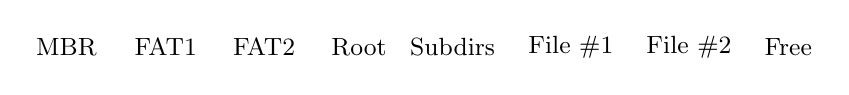
\begin{tikzpicture}[x=.25cm,y=.25cm]
\foreach \y in {1,...,8} {
  \foreach \x in {1,...,40} {
    \dbox{}{\x}{\y}
  }
}
  \Dbox{color=red}{1}{8}  
  \foreach \x in {3,...,4} { \Dbox{color=blue}{\x}{8}  }
  \foreach \x in {5,...,6} { \Dbox{color=green}{\x}{8}  }
  \foreach \x in {7,...,8} { \Dbox{color=pink}{\x}{8}  }
                           { \Dbox{color=cyan}{9}{8} }
  \foreach \x in {11,...,30} { \Dbox{color=yellow}{\x}{8}  }
  \foreach \x in {31,...,40} { \Dbox{color=purple}{\x}{8}  }
  \foreach \x in {1,...,15} { \Dbox{color=purple}{\x}{7}  }

{\small
  \Dbox{color=red}{1}{-1}  ; \node [right] at (1,-1) {MBR};
  \Dbox{color=blue}{6}{-1} ; \node [right] at (6,-1) {FAT1};
  \Dbox{color=green}{11}{-1} ; \node [right] at (11,-1) {FAT2};
  \Dbox{color=pink}{16}{-1}  ; \node [right] at (16,-1) {Root};  
  \Dbox{color=cyan}{20}{-1}  ; \node [right] at (20,-1) {Subdirs};
  \Dbox{color=yellow}{26}{-1} ; \node [right] at (26,-1) {File \#1};
  \Dbox{color=purple}{32}{-1} ; \node [right] at (32,-1) {File \#2};
  \dbox{}{38}{-1} ; \node [right] at (38,-1) {Free};
}
\end{tikzpicture}
\renewcommand*{\dbox}{}
\renewcommand*{\Dbox}{}

\end{center}
\end{figure}

To read the contents of a file on a FAT media the operating system
must decode the structures that make up the file system. This starts
when the computer reads the file system's BPB
to learn the size of the FAT, the size of the root directory, the
cluster size, and other file system parameters. 

Next, the computer will read the first copy of the FAT into
memory. (If there is an error attempting to read the first FAT, it
tries to read the second, and so on.) As mentioned above, the FAT is
an array of 12, 16 or 32-bit integers.  The integers in the FAT don't refer to individual blocks. Instead,
they refer to \emph{clusters}, where a  \emph{cluster} is a contiguous
set of 1, 2, 4, 8 or more disk blocks. The \emph{cluster size} is
file system parameter that is specified when the disk is
formatted. Therefore, a FAT32 file system with a cluster size of 512
(1 sector) has
a maximum file system size of $512\times2{32}=2\textrm{GiB}$, while a
cluster size of 4096 allows for a file system up to 16~GiB. 

The FAT array serves two purposes: it identifies the \emph{allocation
  status} of each cluster---that is, whether the cluster is free and
available for use or if it holds user data. If it does hold user data,
the array tells the operating system how to find each successful
cluster that makes up the file.  For example, if a file occupies
clusters 10 and 11, then slot \#10 in the FAT will contain an |11| and
slot \#11 will contain a special marker that indicates there are no
more clusters in the chain.

Finally, the computer will read the root directory. As mentioned
above, each FAT directory consists of a sequence of 32-byte
records. FAT12 and FAT16 file systems required that file names have a
maximum of 8 characters, a period, and then a 3-character extension,
producing a so-called ``8.3 filename.'' \tabref{table:fatdir} shows
the major elements of the FAT directory entry. FAT32 directory entries
use multiple 32 bytes entries in a row to hold Unicode ``long file
name'' entries that are concatenated together and form an alias for
the short 8.3 file name. The creation and interpretation of long file
names is beyond the scope of this chapter.


\begin{table}
\begin{minipage}{\textwidth}
\caption{The 32 bytes of the FAT directory entry. The first byte
  contains either the beginning of the short file name or a flag
  indicating that the entry is the last or that the entry has been
  deleted and should be ignored. (From Wikipedia, \url{https://en.wikipedia.org/wiki/File\_Allocation\_Table}.)}\label{table:fatdir}
\begin{center}
\begin{tabular}{lll}
\hline
Offset & Length & Description \\
\hline
|00h| & |8| & Short file name (padded with spaces) \\
      & |1| & |00h| -- This is the last entry, and it is available \\
      & |1| & |E5h| -- This entry is deleted; ignore it \\
\hline
|08h| & |3| & Short file extension \\
\hline
|0Bh| & |2| & File attributes and flags\\
\hline
|0Dh| & |1| & Create time miliseconds times 10\\
\hline
|0Eh| & |2| & Create time (bits 15--11:hours; 10--5:minutes; 4--0:seconds)\\
\hline
|10h| & |2| & Create date (bits 15--9:year; bits 8--5:month; bits 4--0: day)\\
\hline
|12h| & |2| & Access date \\
\hline
|14h| & |2| & FAT12 and FAT16: Extended Attributes handle\\

      &     & FAT32: Top 16 bits of cluster with start of file\\
\hline
|16h| & |2| & last write time\\
\hline
|18h| & |2| & last write date\\
\hline
|1Ah| & |2| & Bottom 16 bits of start cluster\\
\hline
|1Ch| & |4| & Size of file\\
\hline
\end{tabular}
\end{center}
\end{minipage}
\end{table}





\subsection{Partitioning and Volume Management}

Although a file system can be stored directly on a drive, with the
first block of the drive being used to store the first block of the
file system, this is not commonly done. Instead, the first 
block of the drive is typically used to store a \emph{disk label} and  \emph{partition
  table} that provides the storage media with a unique identifier and describes the
locations of the file systems that the media contains. Advantages of
this approach include:
\begin{itemize}
\item A single physical device can contain multiple partitions, each
  with its own file system.
\item Partitions can identify specific regions of the disk as reserved
  or encrypted, so that the operating system doesn't inadvertently
  damage them.
\item The device label allows the operating system reference the media
  by name, rather than by location such as the interface or bus. This
  allows computer hardware to be reconfigured without having to update
  operating system configuration.
\end{itemize}

One of the most commonly used partitioning schemes are the
\emph{Master Boot Record} (MBR) format, originally created in 1982 for
the IBM PC/XT and used with minor revisions ever since.

The MBR occupies the first sector of a hard drive used on most
Windows-based computers. When the computer starts up the Basic
Input/Output System (BIOS) loads these 512 bytes into the start of
memory and jumps to location 0. Typically the MBR contains a short
program that loads more sectors from the hard drive into memory and
runs them; this second boot loader loads the operating system and runs
it.

\begin{table}
\begin{minipage}{\textwidth}
\caption{Structure of the Master Boot Record. ({\small from Wikipedia, \url{http://en.wikipedia.org/wiki/Master_boot_record}})}\label{mbr}
\begin{tabular}{|>{\tt}c|>{\tt}c|c|c|c|}
\hline
\multicolumn{2}{|c|}{\bf Address} & \multicolumn{2}{c|}{}                              & \\
\cline{1-2} \bf Hex & \bf Dec         & \multicolumn{2}{c|}{\multirow{-2}{*}{\bf Description}} & \multirow{-2}{*}{\bf Size in bytes}\\
\hline
+000h & +0   & \multicolumn{2}{c|}{Bootstrap code; extended information} & |446| \\
\hline
\hline
+1BEh & +446 & \multicolumn{2}{c|}{Partition entry \#1} & |16| \\
\hline
+1CEh & +462 & \multicolumn{2}{c|}{Partition entry \#2} & |16| \\
\hline
+1DEh & +478 & \multicolumn{2}{c|}{Partition entry \#3} & |16| \\
\hline
+1EEh & +494 & \multicolumn{2}{c|}{Partition entry \#4} & |16| \\
\hline
+1FEh & +510 & |55h| & & \\
\cline{1-3}
+1FFh & +511 & |AAh| & \multirow{-2}{*}{Boot Signature} & \multirow{-2}{*}{2} \\
\hline
\hline
\multicolumn{4}{|r|}{\textbf{Total size: $\bf 446 + (4\times16) + 2 $}} & \textbf{512}\\
\hline
\end{tabular}
\end{minipage}
\end{table}


\begin{table}
\caption{Structure of the 16-byte partition
  entry. {\small(From Wikipedia, \url{http://en.wikipedia.org/wiki/Master_boot_record})}}\label{mbr:partition}
\begin{tabular}{|>{\tt}c|>{\tt}c|l|}
\hline
\textrm{Offset} & \textrm{Length} & Description \\
\hline
+0h & 1 & Status; |80h|:active; |00h|: inactive \\
+1h & 3 & CHS address of first sector in partition (not used on modern systems) \\
+4h & 1 & Partition Type Code \\
+5h & 3 & CHS address of last sector in partition (not used on modern systems)\\
+8h & 4 & LBA address of first sector in partition \\
+Ch & 4 & Number of sectors in partition \\
\hline
+0h & 16 & Total number of bytes in entry \\
\hline
\hline
\end{tabular}
\end{table}

The basic MBR (\tabref{mbr}) provides for four partitions, each
described by a 16-byte partition entry record. The record includes a
byte indicating if the corresponding partition is active or not, the
start of the partition and the partition's length.  Originally the
start and end were encoded as a 3-byte CHS (Cylinder, Head, Sector)
triplet. Today the CHS entries are ignored and the partition is
described with a pair of 32-bit LE numbers conveying the Logical Block
Address (LBA) of each partition's first block and a block
count. Because blocks are assumed to be 512 bytes, this scheme allows
for a maximum media size of $512 \times 2^{32}=2\textrm{TiB}$ in
storage.

The MBR was first introduced by
IBM PC DOS 2.0 in 1983. Since then there have been at least six different
versions of the MBR
used\footnote{\url{http://en.wikipedia.org/wiki/Master_boot_record}}. ALl
of the MBRs store bootstrap code
at location |0|, place the first four partition entries starting at location
|1BEh|, and have a boot signature in the last two blocks of the
sector. This consistency provides for backwards compatibility,
allowing each generation of disk utilities and BIOS drivers to make
sense of whatever data they might find on a mass storage device.
Modern computers use a new partitioning scheme called the GUID
Partition Table
(GPT)\footnote{\url{http://en.wikipedia.org/wiki/GUID_Partition_Table}},
but even these systems include something called a ``Protective MBR''
that allocates the entire drive to a partition of type |EEh|. As its
name implies, this partition protects the GPT disk in the event that
the user attempts to mount it on a system that does not understand GPT
partitioning: instead of inadvertently overwriting the GPT partition,
the non-GPT system will leave it alone, since the entire media is in
use by a partition type that the non-GPT system does not understand.


\subsection{Flash Memory, Solid State Drives, and the Flash Translation Layer}

Flash memory storage was introduced to consumers in the 1990s as a
data storage system for digital cameras, digital audio players, and
personal digital assistants. Flash storage is
similar to magnetic storage systems in that flash is \emph{non-volatile} and block
addressable. It is different in that blocks are grouped into
\emph{pages} that be explicitly erased
as a set before the individual blocks can be rewritten, and each block
experiences \emph{wear} each time it is erased, and as a result each
block can only be rewritten finite number of times before it
fails. Typically this limit is between a thousand and a hundred
thousand rewrites. Despite these limitations, flash has
steadily grown in popularity because of its physical durability (there
are no moving parts), its speed of access (no seek time), and its
steadily increasing storage capacities.

Because file systems like FAT tend to repeatedly rewrite a small
number of sectors used for file system metadata (e.g. the file
allocation table), these file systems cannot be used directly with
flash storage: doing so would cause the ``hot'' blocks holding the
rapidly changing metadata to wear out, since the metadata needs to be
updated each time a file is created or deleted. In a digital camera
application, for example, blocks devoted to the File Allocation Table
would be destroyed after only a few thousand photographs had been
taken, creating a media with an unacceptably short lifespan.

Modern flash storage systems get around this problem with a technique
called wear leveling. The flash storage device implements a
\emph{Flash Translation Layer} that maps the logical block address
viewed by the operating system to the physical flash page used by the
storage device. Each time a block is rewritten, the new data are
written to a new physical locations. Periodically
the FTL writes a new \emph{translation table} to the device with the
mapping. As a result, writes to hot blocks such as the FAT are cycled
through the physical storage device, and instead of being able to
handle thousands of rewrites, the flash device can accommodate 
thousands of billions. 

Although in theory it is possible to access to physical storage of a
flash device, in practice the FTL hides the physical layer and allows
access only to the logical blocks.

\subsection{Encrypting File Systems}

Adding to the complexity of the is \emph{encryption}, which can be
applied at nearly any location between the user and the storage
media. Using encryption provides a significant layer of security: with
encryption, the data on the storage system can be accessed but not
understood unless the appropriate decryption key is available.

Encryption is very flexible. It can be within the storage device itself (as in the case of an
encrypting hard drive), in the operating system's disk driver, in the logical volume
management system, in the file system, or at the application level. 

Encryption is discussed in \chapref{ch:encryption}.


\subsection{Putting it all together: A 128~MB FAT16 Disk Image}
In this section we will explore the contents of an SD camera card
created in 2013 with a Canon PowerShot SX260~HS camera. The card is called NPS-2009-CANON2.

To create the data for this section, we started with a 128MB camera
card and cleared every addressable sector by overwriting that sector's
content with NULL bytes. We did this by inserting it into a Linux
computer. Inserting the card caused Linux to create two devices in the
|/dev| file system:

\begin{tabular}{ll}
|/dev/sdb| & Virtual device for the entire physical volume \\
|/dev/sdb1| & Virtual device for the first partition \\
\end{tabular}


We then unmounted the FAT16 file system and wiped the physical volume
with these commands:

\begin{code}
$ (@ \sl{sudo umount /dev/sdb1} @) 
$ (@ \sl{sudo dd if=/dev/zero of=/dev/sdb} @)
\end{code}
%$

This |dd| command is conceptually similar to the program in Listing\ref{clear.py}.

You can do this
easily with the program in \figref{overwrite}.

\lstinputlisting[caption=\textbf{clear.py}: A simple program to clear a disk.]{ch-drives/clear.py}\label{clear.py}

After the card was cleared, we put it into the PowerShot, initialized
the card, took two photos, deleted the first with the camera, and then
removed the card and put it back in the same Linux computer. Finally
we used the |dd| command a second time to copy the raw blocks into a
disk file, creating a \emph{disk image}:\footnote{You can download that file
from \url{http://digitalcorpora.org/corp/nps/nps-2013-canon1/nps-2013-canon1.raw}}

\begin{code}
$ (@ \hl{sudo umount /dev/sdb1} @)
$ (@ \hl{sudo dd if=/dev/sdb of=nps-2013-canon1.raw conv=noerror,sync} @)
\end{code} 

The |dd| command copies blocks of data from the input file (\emph{if=})
to the output file (\emph{of=}). Two conversion options are
specified: \emph{noerror} tells the \emph{dd} command to continue even
if it encounters an error, and \emph{sync} tells the program to keep
the output stream synchronized with the input stream in the event of
an error by writing blocks filled with NULLs.  Notice that each time we unmounted the file system but imaged the
entire drive. In this way we get the partition table and the slack
space before the beginning of the first file system.  


\subsection{Viewing canon1's MBR}

\figref{fig:fat16l} shows a conceptual view of
canon1's storage. The card has a Master Boot Record in its
first sector (block |0|) which has two slots: slot 1 is an unallocated
region between blocks |0| and |96| (including, somewhat confusingly, the
master boot record itself). Slot |2| is a DOS FAT16 file system that
occupies blocks |97| through |250879|. The FAT file system contains its own
structures, including a \emph{Boot Sector Structure} that describes the
file system, a \emph{root directory}, \emph{subdirectories},
\emph{files}, and finally a \emph{file allocation table} that both
describes which sectors belong to which file and indicates which
sectors are free and available for new files. We'll discuss each of
those in the following section.


You can display the contents of the MBR by viewing a hex dump of the
first sector:

\begin{code}
$ (@ \hl{xxd -a -len 512 nps-2013-canon1.raw} @)
0000000: 0000 0000 0000 0000 0000 0000 0000 0000  ................
*
00001b0: 0000 0000 0000 0000 0000 0000 0000 0003  ................
00001c0: 0200 0607 e0d3 6100 0000 9fd3 0300 0000  ......a.........
00001d0: 0000 0000 0000 0000 0000 0000 0000 0000  ................
00001e0: 0000 0000 0000 0000 0000 0000 0000 0000  ................
00001f0: 0000 0000 0000 0000 0000 0000 0000 55aa  ..............U.
$ 
\end{code}

The |-a| option tells the |xxd| command to suppress identical lines
from the first line (that is, lines that contain 16 NULLs), the \texttt{-len~512} tells the command to only display the first 512 bytes of the
file, and |nps-2013-canon1.raw| is the file name.

Decoding this output is not difficult but can be time consuming. Instead of
manually attacking the hex values, it is more effective to write a
program that does this work for you. Listing~\ref{mbrdecode} the start
of such a program in Python. This program  will open
up the disk image, read the sector into memory, and then print the
fields. 

\begin{figure}
\lstinputlisting[caption=The start of a python program to display the
  Master Boot Record.]{ch-drives/mbrdecode.py}\label{mbrdecode}
\end{figure}

Finally, you can view the contents of the MBR using the SleuthKit's |mmls| command:

\begin{code}
$ (@ \hl{mmls /corp/nps/drives/nps-2013-canon1/nps-2013-canon1.raw} @)
DOS Partition Table
Offset Sector: 0
Units are in 512-byte sectors

     Slot    Start        End          Length       Description
00:  Meta    0000000000   0000000000   0000000001   Primary Table (#0)
01:  -----   0000000000   0000000096   0000000097   Unallocated
02:  00:00   0000000097   0000250879   0000250783   DOS FAT16 (0x06)
$ 
\end{code}

Use the \texttt{-h} option to display all of the options that your
version of the |mmls| command supports.


The first block of a FAT file system contains a \emph{Boot Sector
  Structure} that describes the file system's parameters, including
the sector size, the cluster size, the number of reserved sectors, the
number of File Allocation Tables, and so on. The layout of this
structure is described in Microsoft's FAT specification; you can also
find it in the SleuthKit file |tsk3/fs/tsk_fs.h|\footnote{The current
  version of this file can be found at \url{https://github.com/sleuthkit/sleuthkit/blob/master/tsk3/fs/tsk_fs.h}.}. The first
few lines of the SleuthKit structure are show in \figref{BSS}.

\begin{lstlisting}[caption={The first few bytes of the Boot Sector
      Structure, the first sector of a FAT file system. From
      Sleuthkit's \texttt{tsk\_fs.h}.\label{BSS}}]
/*
 * Boot Sector Structure for TSK_FS_INFO_TYPE_FAT_12,
 * TSK_FS_INFO_TYPE_FAT_16, and TSK_FS_INFO_TYPE_FAT_32
 */
    typedef struct {
        uint8_t f1[3];
        char oemname[8];
        uint8_t ssize[2];       /* sector size in bytes */
        uint8_t csize;          /* cluster size in sectors */
        uint8_t reserved[2];    /* number of reserved sectors for boot sectors */
        uint8_t numfat;         /* Number of FATs */
        uint8_t numroot[2];     /* Number of Root dentries */
        uint8_t sectors16[2];   /* number of sectors in FS */
        uint8_t f2[1];
        uint8_t sectperfat16[2];        /* size of FAT */
        uint8_t f3[4];
        uint8_t prevsect[4];    /* number of sectors before FS partition */
        uint8_t sectors32[4];   /* 32-bit value of number of FS sectors */

        /* The following are different for fat12/fat16 and fat32 */
        ...
\end{lstlisting}

Because the FAT file system begins in sector |97|, the number |97|
must be added to all internal references. Typically this is done in
the device driver, since the device driver must be aware of the disk
partitioning scheme.   

From the parameters stored at sector |97| it is possible to
calculation the location of each of the parts mentioned above.  The
first fat is stored at an offset specified by |reserved|, which must
be interpreted as a 16-bit LE number.  The space allocated by the FATs
is equal to the number of FATs times the number of sectors per
FAT. The number of sectors taken up by the root directory is equal to
the number of root entries times 32 divided by the number of bytes per
sector. Finally there is the data region, which is the start of
cluster \#2. (Cluster numbers 0 and 1 are reserved.)

\section{Exercise: Windows - Creating and Testing FAT32 Disks}

This exercise is designed to help you understand how file systems
store information and the opportunities for retaining
privacy-sensitive information that is not visible to the user. 

This exercise will be done with a \emph{virtual disk}. Like a physical
mass storage device, a virtual disk consists of a set of numbered data
blocks. But instead of storing those blocks directly in on a mass
storage device, the blocks are stored in another file. The operating
system treats the virtual disk like a physical drive: it can be
formatted, files can be copied to it, and so on. But we can also
access the underlying file that holds the virtual disk. This makes it
easier to inspect the individual data blocks.

We will use the Windows |DISKPART| command to create and manage virtual
disks. |DISKPART| is a command-line tool that needs to run as
Administrator.

We will be using these commands:

\begin{tabular}{>{\tt}ll}
\hline
help partition & shows partition command available\\
create vdisk & Creates a virtual disk \\
list disk & Shows available disks \\
list vdisk & Shows detailed information about the available VDisks\\
list partition & Shows available partitions \\
\hline
\end{tabular}

We will create a text file on the virtual disk that has a sensitive file
name and file contents. Next we will take a screen shot and save it on
the computer's hard drive as a JPEG. We will then delete the text file
and empty the trash. Finally we will inspect the disk image and see if
we can find the text file and the screen shot.


\begin{enumerate}


\item Click the Start button, type |diskpart| into the search field,
and click on the |diskpart| program icon.
\item The User Account Control will ask you to verify that you want to
run the DiskPart, a program that can make ``changes to the computer.''
Click ``Yes.''  The |diskpart.exe| window should appear.
\item If you haven't done so already, right-click on the window's
titlebar and select ``Properties.'' Click on the Layout tab and change
the ``Screen Buffer Size'' to 9999. This will allow you to scroll
backwards and see the entire history of your DISKPART session.
\item Type |help| to see the list of commands that the DISKPART
command supports. You may need to make the window larger.

\item Create a 16MB virtual disk with the command:

\begin{code}
DISKPART> (@ \hl{create vdisk file="C:\textbackslash{}disk1.vhd" maximum=16} @)
\end{code}

\item Attach the disk you just created:
\begin{code}
DISKPART> (@ \hl{attach vdisk} @)
\end{code}

\item Verify that the disk is attached:
\begin{code}
DISKPART> (@ \hl{list disk} @)
...
DISKPART> (@ \hl{list vdisk} @)
\end{code}

\item Now we need to create a partition, assign a letter to that
partition, and format the drive. We will call this drive K: and format
it with FAT. 
\begin{code}
DISKPART> (@ \hl{create partition primary} @)
DISKPART> (@ \hl{assign letter=k} @)
DISKPART> (@ \hl{format fs=fat label="WORK"} @)
\end{code}
\end{enumerate}

At this point we have a 16MB virtual disk attached to the computer as
drive K:. The drive's contents are stored in the file |C:\disk1.vhd|.

Lastly, we want to put a file on this disk. For test purposes we are
going to use a small file with a distinctive file name and file
contents.

\begin{enumerate}[resume]
\item Run the windows NotePad program by clicking the Start program,
typing ``Notepad'' into the search field, and clicking on the icon.

\item Type this text into the document:  ``The phone number is
202-555-1212.'' You can use your own phone number and add additional
information if you wish.

\item Select ``File/Save As'' and save the file on the WORK (K:) drive
with the name ``file-name-example-0001.txt''. 

\item Close the Notepad program.

\item Now we will detach the virtual disk:

\begin{code}
DISKPART> (@ \hl{detach vdisk} @)
\end{code}

\end{enumerate}

\subsection{Looking for the files}
The 

\section{Working with Disk Images}

Today there are three fundamental kinds of forensic data:

\begin{itemize}
\item Disk Images
\item Memory Images
\item Packets intercepted on a network.
\end{itemize}

Most research to date has been done with Disk images. Most data is
stored on disk, and most forensic investigations have been for the
purpose of finding information that is on a disk (such as in the case
of a child pornography investigation), or in trying to understand
information left behind on a disk (for example, after an intrusion or
malware incident.

It is also common to find the other kinds of information on disk
images. Memory is frequently stored on disk images from swapping
(e.g. PAGEFILE.SYS on Windows) or system hibernation
(HIBER.SYS). Packets are found on image files when the disks were used
to store the results of a network interception.

Working with image files can consists of these activities:


\begin{itemize}
\item Copying the data from the source drive into the image file, a
  process called \emph{drive imaging}.
\item Computing the checksum of the disk image.
\item Validating the copy against the original.
\item Creating a digital signature for the disk image.
\item Self-validating the copy.
\item Making backup copies of the disk image, and validating the integrity
  of the backups.
\item Converting the disk image into a form that can be used by your
  forensic tool
\end{itemize}.

On the \url{digitalcorpora.org} website there are several disk images with
which you can work. We're going to do our initial work with the image
nps-2009-canon2-gen6. This image is usually stored in the directory
/corp/drives/nps/nps-2009-canon2/.

The nps-2009-canon2 disk images are a series of images created with a
Canon digital camera and a 32MB SD card. First the card was
\emph{cleared} using |dd| on a Linux computer. The card was then
inserted into the digital camera, a series of photos were taken, and
the card was removed and imaged. The card was put back into the
camera, some of the photos were deleted, and new photos were
taken. This process was repeated five times, creating a total of six
disk images, nps-2009-canon2-gen1 through nps-2009-canon2-gen6.

The SD card contained 60,800 512-byte sectors, for a total of
31,129,600 bytes (30,400 KiB).

For each disk image four files are distributed:

   .raw -- a raw disk image that's 31,129,600 bytes in length
   .E01 -- An EnCase E01 file of the disk image
   .xml -- A digital forensics XML file describing the files resident
           in the disk image.


It is customary in digital forensics to use cryptographic hashes to
verify the integrity of a disk image. When the disk is first imaged
the hash is recorded in a secure manner (typically written in in
investigator's notebook). From that point forward, the image can be
manually validated by recomputing the hash and comparing it to the
original recording.

The hash of a raw file can be easily calculated the ``openssl''
command:

\begin{Verbatim}
$ openssl md5 /corp/drives/nps/nps-2009-canon2/nps-2009-canon2-gen6.raw
MD5(/corp/drives/nps/nps-2009-canon2/nps-2009-canon2-gen6.raw)=750b509d8fbed37a5213480aaccfdc61
$ 
\end{Verbatim}

You can't calculate the hash of an E01 file in this manner,
however, because these files contain additional metadata that is not
part of the disk image.  Both of these formats also store hash codes
directly in the disk image. This allows you to \emph{validate} the
contents of a disk image with a command that calculates the hash by
examining the data and comparing it with the stored value. 

\subsection{E01 files}
You can use the ewfinfo command to view the metadata information of a
disk image:

\begin{Verbatim}
% ewfinfo /corp/drives/nps/nps-2009-canon2/nps-2009-canon2-gen6.E01 
ewfinfo 20090927 (libewf 20090927, libuna 20090901, libbfio 20090927, zlib 1.2.3, libcrypto 0.9.8)

Acquiry information
Acquiry date:Mon Apr 12 08:12:32 2010
System date:Mon Apr 12 08:12:32 2010
Operating system used:Darwin
Software version used:20090927
Password:N/A

EWF information
File format:EnCase 6
Sectors per chunk:64
Error granularity:64
Compression type:no compression
GUID:dc032794-bef0-2c45-8ede-8cc01ed31683

Media information
Media type:removable disk
Is physical:no
Bytes per sector:512
Amount of sectors:60800
Media size:29 MiB (31129600 bytes)

Digest hash information
MD5:750b509d8fbed37a5213480aaccfdc61

% 
\end{Verbatim}


You can verify the contents of an E01 file using the ewfverify
command:

%% BEGIN NO FILL
\begin{Verbatim}
$ ewfverify /corp/drives/nps/nps-2009-canon2/nps-2009-canon2-gen6.E01 
ewfverify 20090927 (libewf 20090927, libuna 20090901, libbfio
20090927, zlib 1.2.3, libcrypto 0.9.8)

Verify started at: Mon Jun  7 14:20:20 2010

This could take a while.

Status: at 0%.
        verified 32 KiB (32768 bytes) of total 29 MiB (31129600 bytes).

...

Status: at 100%.
        verified 29 MiB (31129600 bytes) of total 29 MiB (31129600 bytes).

Verify completed at: Mon Jun  7 14:20:20 2010

Read: 29 MiB (31129600 bytes) in 0 second(s).

MD5 hash stored in file:750b509d8fbed37a5213480aaccfdc61
MD5 hash calculated over data:750b509d8fbed37a5213480aaccfdc61

ewfverify: SUCCESS
$ 
\end{Verbatim}
%% END NO FILL




\subsection{Exercises}
\begin{itemize}
\item Download an install the following programs in this order:
\begin{itemize}
\item   libewf
\item  sleuthkit
\end{itemize}
\item Download nps-2009-canon2-gen6.e01 and nps-2009-canon2-gen6.raw
\item Verify the SHA1 of each file. Verify the RAW with the openSSL
  command and make sure that it matches what is in this book. Use the
  ewfverify and afverify commands to verify that the hash codes stored
  in the E01 files match the computed values.
\item Convert the RAW file to an E01 files. Notice that the
  files are different than the distribution E01 files.
\item Verify your converted files.
\item Convert the distribution E01 files back to raw files and
  use the Unix |cmp| command to show that the resulting files match
  the distribution raw file.
\end{itemize}


\section{Going Deeper}
\subsection{File Systems of Interest}
There are a many different kinds of file systems in use on
modern computer systems:
\begin{description}
\item[Disk file systems] organize files and directories on
  block-oriented storage systems. 
\item[Memory file systems] implement a file abstraction in
  memory. Such systems can provide for increased performance when
  compared to using a conventional file system on a simulated block
  device. One of the most common examples of a memory file system is tmpfs\cite{Snyder90tmpfs:a}.
\item[Distributed file systems] allow a computer to access
  information on remote servers as if it is stored
  locally. Distributed file systems are forensically interesting
  because many use local storage to cache information from the remote
  servers. Analyzing local storage can therefore give clues as to what
  was accessed remotely, and when it was accessed. Examples of
  distributed file systems include Sun's Network File System
  (NFS)\cite{Sandberg85designand,Pawlowski00thenfs} and Microsoft's
  Common Internet File System (CIFS)\cite{ms-cifs}.
\item[Virtual file systems] use the file and directory abstraction to
  make it easy to access other information. For example, the Linux
  |/dev| file system is used to access devices through the file
  system, the |/sys| file system is used to access features within
  the system kernel, and the |/net| file system accesses the
  automounter. Virtual file systems are not typically of interest in
  MEDEX because they do not leave residual information on a storage
  device. However, virtual file systems are relevant in malware
  analysis and intrusion response.
\end{description}

As this chapter is written, the following file systems are of general
interest. The number after each file system is date that the file
system became made generally usable:
\begin{description}
\item[FAT12, FAT16 and FAT32 (1980)] file systems developed by Microsoft for use with
  DOS and early versions of Windows. 
  
\item[HFS, HFS+ (1985)] the Hierarchical File System, developed by Apple
  Computer and introduced with the first Macintosh hard
  drive. Whereas most file systems of the time used tables and arrays to store
  information, HFS and HFS+ use b-trees.
\item[NTFS (1993)] the New Technology File System, developed by
  Microsoft for use with Windows NT. 
\item[EXT2/3/4 (1993)] The extended file system, developed for use with Linux systems.
\item[exFAT (2007)] a modification of the FAT file system designed to
  support large files and optimized for use on flash drives.
\item[YAFFS, YAFFS2 (2002)] ``Yet another flash file system,'' a file
  system specifically designed for use with NAND flash chips found in
  cell phones. Unlike other file systems, YAFFS2 specifically adapts
  to the requirement that flash pages be cleared before they can be
  re-written. It also handles wear-leveling and garbage collection.
  YAFFS2 gained popularity through its use in Android, although it is
  increasingly being replaced through the use of proprietary flash
  translation layers (FTLs).
\end{description}

SleuthKit version 4.1 provides read-only support for all of the file
systems listed above. Read-write support for the file systems is
inconsistent, with most operating systems supporting FAT and NTFS,
but support for others being inconsistent.

Confusingly, the phrase \emph{file system} is used ambiguously to
describe both the organization of data on a mass storage device and
the code that implements the file abstraction. Thus, are multiple FAT
implementations, only some of which are authored by
Microsoft. Different file system implementations are supposed to be
mutually compatible, but because of the complexity inherent in
creasing a file system implementation, incompatibilities inevitability
emerge.

Any computational storage device or storage abstraction can be used to
virtualize and contain any other storage device. That is, a file can
be stored in a file system, but a file system can also be created and
stored inside a file (this is essentially what a disk image is). For
example, it is possible to create a USB drive that boots a copy of
Linux but also functions under Windows: The Linux EXT file system is
stored inside a rather large file in an outer FAT32 file system.

\subsection{Books}
\subsection{Articles}
\subsection{Web Sites}
\url{http://www.pjrc.com/tech/8051/ide/fat32.html}
\subsection{Wikipedia}
As of this writing, the following wikipedia pages provide excellent
insight to the concepts mentioned in this chapter:

\begin{description}
\item[\href{http://en.wikipedia.org/wiki/Copy-on-write}{Copy-on-write}]
\item[\href{http://en.wikipedia.org/wiki/Logical_Unit_Number}{Logical
    Unit Number}] Something about the LUN
\item[\href{http://en.wikipedia.org/wiki/Logical_volume_management}{Logical
    Volume Management}]
\item[\href{http://en.wikipedia.org/wiki/Snapshot_(computer_storage)}{Snapshot
    (Computer Storage)}]
\end{description}

\section{Terminology}
\sgraphic{art/diskpart-1}{The Windows diskpart command is used to create and
  manage physical and virtual disks.}


Allocated

Blocks

Carving

Clusters

Deleted

File Allocation Table

Free List

inode

Hard Link

Symbolic Link

Master File Table

Overwritten

TRIM Command

Undelete

Unlink

\section{Exercises---Operating Systems}
This problem set assumes that you have read the draft ``Finding Hidden Data
in File Systems'' chapter of \emph{Technical Privacy Auditing with
  Computer Forensics Tools}

\begin{enumerate}
\item Download canon1\footnote{\url{http://digitalcorpora.org/corp/nps/nps-2013-canon1/nps-2013-canon1.raw}} and show a hex dump of the
  images' first sector.
\item Draw a box around hex bytes in the dump that
  correspond to the first slot in the partition table.
\item Run \texttt{mbrdecode.py} (\ref{mbrdecode}) on Canon1 and provide the results.
\item The first block of Canon1's FAT16 partition contains a Boot
  Sector Structure. Extend \texttt{mbrdecode.py} to read this block
  and print the fields. 
\item Further extend \texttt{mbrdecode.py} to print the contents of the root
  directory.  You will do this by:
\begin{enumerate}
  \item Determining the location and length of the root directory
    from the BSS.
  \item Reading the root directory into a buffer.
  \item Creating a function that takes a buffer and prints each
    directory entry that the buffer contains.  This function will
    operate by stepping through the buffer 32 bytes at a time.
\end{enumerate}  

\item In order to work with files it is necessary to read the File
  allocation table. Using the information you learned in the previous
  step, provide the sector numbers where the FAT starts and stops.
\end{enumerate}

\noindent   Recall that sectors on a FAT volume used to hold user data are
  called \emph{clusters};  each cluster may consist of one or
  more sectors (blocks). Each file can therefore be referred to by the
  number of the cluster where the first byte of file data is
  stored. The FAT array for each cluster contains a pointer to the
  location of the next cluster or a special value indicating there are
  no more data clusters. Each file is therefore described by a linked
  list of cluster numbers, and all of the linked lists for all of the
  files are stored within the fAT.

\begin{enumerate}[resume]
\item Modify the \texttt{mbrdecode.py} program to read the
  entire FAT into an integer array. 
\end{enumerate}
  
\noindent  The remainder of these problems work with two
  files. File \#517 is the
  directory \verb|\DCIM\111___06\| while File \#1030 is the JPEG image
  \verb|IMG_0126.JPG| in that directory.

\begin{enumerate}[resume]
\item  Once you have modified \texttt{mbrdecode.py} to read the entire FAT
  into memory, modify it further to print all of the cluster numbers 
  associated with File \#517. Provide a list of the clusters.

\item Provide a list of the clusters associated with File \#1030.

\item Now that you have a list of data clusters, you can read the
  contents of the files and decode them!  Read File \#517 into a
  buffer and print its contents using the function you wrote that
  decodes file directories. Provide this output and explain each entry.

\item Read File \#1030 and store the results in a file on your host
  computer called \emph{FILE1030.jpg}. Show the contents of that file graphically.

\end{enumerate}
  
\noindent Extra credit:


\begin{enumerate}[resume]
\item Write a program that starts at the root
  directory and recursively lists the name, modification date, and
  size of every file on the disk.
\item Create a virtual disk using the instructions in the chapter. Put
  a few files on the disk and delete a few of them. Read the directory
  and explain which files can be recovered with file recovery
  utilities. Write a file recovery utility and try to recover one or
  more of the deleted files.
\end{enumerate}




\section{Exercises}

\begin{enumerate}
\item Download GEN1 (nps-2009-canon2-gen1.raw) and show a hex dump of the
  images' first sector.
\item Draw a box around hex bytes in the dump that
  correspond to the first slot in the partition table.
\item Show a hex dump of the GEN1 Boot Sector Structure.
\item Run the \texttt{mbrdecode.py} program shown in the chapter on
  GEN1 and provide the results.
\item Extend \texttt{mbrdecode.py} to decode and print all of the
  fields in the Boot Sector Structure. You will do this by:
\begin{enumerate}
  \item Determining the block number in which the BSS resides. (Hint:
    it's the first block of the partition.)
  \item Reading the block into a buffer.
  \item Using \texttt{struct.unpack} to decode the buffer. (You
  can do this in a single statement or with a series of statements as
  we do in the Listing.)
  \item Printing each value. 
\end{enumerate}


\item Extend \texttt{mbrdecode.py} to print the contents of the root
  directory.  You will do this by:
\begin{enumerate}
  \item Determining the location and length of the root directory
    from the BSS.
  \item Reading the root directory into a buffer.
  \item Creating a function that takes a buffer and prints each
    directory entry that the buffer contains. 
\end{enumerate}  

\item In order to work with files it is necessary to read the File
  allocation table. Using the information you learned in the previous
  step, provide the sector numbers where the FAT starts and stops.

\item Modify the \texttt{mbrdecode.py} program to read the
  entire FAT into an integer array. 

  Recall that sectors on a FAT volume used to hold user data are
  called \emph{clusters};  each cluster may consist of one or
  more sectors (blocks). Each file can therefore be referred to by the
  number of the cluster where the first byte of file data is
  stored. The FAT array for each cluster contains a pointer to the
  location of the next cluster or a special value indicating there are
  no more data clusters. Each file is therefore described by a linked
  list of cluster numbers, and all of the linked lists for all of the
  files are stored within the fAT.

  For the remainder of this problem set we will be working with two
  files. File \#517 is the
  directory \verb|\DCIM\100CANON\| while File \#1029 is the JPEG image
  \verb|IMG_0001.JPG| in that directory.

  Once you have modified \texttt{mbrdecode.py} to read the entire FAT
  into memory, modify it further to print all of the cluster numbers 
  associated with File \#517. Provide a list of the clusters.

\item Provide a list of the clusters associated with File \#1029.

\item Now that you have a list of data clusters, you can read the
  contents of the files and decode them!  Read File \#517 into a
  buffer and print its contents using the function you wrote that
  decodes file directories. Provide this output.

\item Read File \#1029 and store the results in a file on your host
  computer called \emph{FILE1029.jpg}. Show the contents of that file.

\end{enumerate}
  
Extra credit:


\begin{enumerate}
\item Write a program that starts at the root
  directory and recursively lists the name, modification date, and
  size of every file on the disk.
\item Create a virtual disk using the instructions in the chapter. Put
  a few files on the disk and delete a few of them. Read the directory
  and explain which files can be recovered with file recovery
  utilities. Write a file recovery utility and try to recover one or
  more of the deleted files.
\end{enumerate}





% LocalWords:  virtualize repurpose
